\documentclass{standalone}
\usepackage{chez}

\begin{document}
%\chapter{November 14, 2019}
There is a more interesting fact though.
\begin{proposition}<nl_subset_p>
  \(\mathsf{NL} \subseteq \mathsf{P}\).
\end{proposition}
Unfortunately if we try to use Savitch's theorem, we get
\(\mathsf{NL} \subseteq \SPACE((\log n)^2)
              \subseteq \TIME(n^{(\log n)^2}) \nsubseteq \mathsf{P}\).
\begin{proof}
  Suppose we have some \textsf{NTM} \(N\) that runs in \(O(\log n)\) space.
  We would like to find some \textsf{TM} \(M\) that runs in polynomial time.

  Given some input \(w\),
  consider the \vocab{computation graph} of \(N\) on \(w\),
  where the nodes are configurations of \(N\) on \(w\),
  and the edges connect \(C_i \to C_j\) if \(C_i\) yields \(C_j\)
  according to the rules of \(N\).
  The number of nodes is polynomial in \(n\),
  so the graph is polynomial in size.
  Therefore, our machine \(M\) can create this graph.

  Now, since \(\textit{PATH} \in \mathsf{P}\),
  we can test if there exists a path from
  \(C_{\textsc{start}}\) to \(C_{\textsc{accept}}\) in the graph.
  If yes then \textsc{accept}, else \textsc{reject}.
\end{proof}

This means that we have the chain of complexity classes
\[
  \mathsf{L} \subseteq \mathsf{NL}
             \subseteq \mathsf{P}
             \subseteq \mathsf{NP}
             \subseteq \mathsf{PSPACE} = \mathsf{NPSPACE}.
\]
Similar to \(\mathsf{P}\) and \(\mathsf{NP}\),
the problem of whether \(\mathsf L = \mathsf{NL}\) is also open.

\subsection{\texorpdfstring{\(\mathsf{NL}\)}{NL}-completeness}
\begin{definition}
  A \vocab{log-space transducer} is a \textsf{TM} that has a read-only input,
  a write-only output, and a work tape that is \(O(\log n)\) space.
  We then say that \(A\) is \vocab{log-space reducible} to \(B\),
  denoted \(A \logredu B\) if there is some function \(f\)
  computable by a log-space transducer such that \(w \in A \iff f(w) \in B\).
\end{definition}

\begin{definition}
  A problem \(B\) is \vocab{\(\mathsf{NL}\)-hard} if
  for all \(A \in \mathsf{NL}\), we have \(A \logredu B\).
  Then, \(B\) is \vocab{\(\mathsf{NL}\)-complete}
  if we also have \(B \in \mathsf{NL}\).
\end{definition}

Let's look at a proposition that we would expect to be true.
\begin{proposition}
  If \(A \logredu B\) and \(B \in \mathsf{L}\), then \(A \in \mathsf{L}\).
\end{proposition}
To prove this, we might try to take a \textsf{TM} \(R\)
that decides \(B\) in \(O(\log n)\) space,
and then construct the \textsf{TM} \(S\) that does the following:
\begin{enumerate}[start=0]
  \item On input \(w\):
  \item Run \(f\) on \(w\) to get \(f(w)\).
  \item Test using \(R\) if \(f(w) \in B\).
        If yes then \textsc{accept},
        else \textsc{reject}.
\end{enumerate}
However, this does not work!
\(R\) does not have enough memory to store the value of \(f(w)\).
Luckily, there is an easy fix to this.
In particular, we just don't store the value of \(f(w)\),
and we compute \(f(w)\) every time to get the part we need.
In particular, let \(f(w, i)\) be the \(i\)th bit of \(f(w)\).
Note that this is also computable in \(\log\) space.
We can just request \(f(w, i)\) whenever we need the \(i\)th bit of \(f(w)\).
\begin{proof}
  Let \(f(w, i)\) be the function computable in log space
  that gives the \(i\)th bit of \(f(w)\),
  where \(f\) is the reduction for \(A \logredu B\).
  Then, consider the following \textsf{TM} that runs in \(\log\) space:
  \begin{enumerate}[start=0]
    \item On input \(w\):
    \item Simulate the decider for \(B\) on an abstract input \(x\).
    \item When the decider asks for the \(i\)th bit of \(x\),
          give it \(f(w, i)\).
    \item Return whatever the decider returns.\qedhere
  \end{enumerate}
\end{proof}

\begin{theorem}
  \(\textit{PATH}\) is \(\mathsf{NL}\)-complete.
\end{theorem}
\begin{proof}
  We showed earlier that \(\textit{PATH} \in \mathsf{NL}\).
  To show that \(\textit{PATH}\) is \(\mathsf{NL}\)-complete,
  suppose \(A \in \mathsf{NL}\).
  Then, we want to find a log-space reduction
  \(f \colon w \mapsto \angles{G, s, t}\)
  where \(w \in A \iff \angles{G, s, t} \in \textit{PATH}\).
  As in \cref{prop:nl_subset_p}, we can let \(G\) be the computation graph,
  \(s = C_{\textsc{start}}\), and \(t = C_{\textsc{accept}}\).

  It suffices to show that we can compute \(f\) in log space.
  Each state in \(G\) can be represented in \(O(\log n)\) space.
  For the edges, we must determine
  whether one state goes to another in log space.
  This works because we only have to analyze two states at a time,
  which can be stored in \(O(\log n)\) space.
\end{proof}

We have another surprising result.
In general, people believe that
\(\mathsf{P} \subsetneq \mathsf{NP} \intersect \mathsf{coNP}
             \subsetneq \mathsf{NP}, \mathsf{coNP}\)
and \(\mathsf{NP} \neq \mathsf{coNP}\).
However, the analogous statement for logarithmic space is not the same!
In particular, we have the following theorem:
\begin{theorem}
  \(\mathsf{NL} = \mathsf{coNL}\).
\end{theorem}
\begin{proof}
  We proceed by proving that \(\ol{\textit{PATH}} \in \mathsf{NL}\).
  Consider some instance \(\angles{G,
  s, t}\) of \(\ol{\textit{PATH}}\), where \(G = (V, E)\).
  Let
  \[
    R = \set{u \mid \text{vertex $u$ is reachable from $s$}}
  \]
  and \(c = \size R\).
  The idea is that if we know \(c\), then we can find \(c\) reachable nodes,
  and if \(t\) is not in the set, we accept.
  To do this, we can iterate through the nodes,
  and nondeterministically guess whether a node \(u\) is reachable or not.
  If we guess that it is reachable,
  then we will try to find a path using
  the same method we used to show that \(\textit{PATH} \in \mathsf{NL}\).

  Now it suffices to find \(c\).
  To do this, we will let \(R_i\) be the set of nodes
  reachable from \(u\) in \(i\) steps, and let \(c_i = \size{R_i}\).
  If \(\size V = m\), we have
  \[
    R_1 \subseteq R_2 \subseteq R_3 \subseteq \dots \subseteq R_m = R.
  \]

  Consider the following nondeterministic
  inductive procedure to find \(c_m = c\).
  We know that \(c_0 = 1\).
  To find \(c_{i + 1}\) from \(c_i\),
  we will check both \(R_i\) and \(R_{i + 1}\).
  In particular, for each potential node \(v \in V\) of \(R_{i + 1}\),
  we find all nodes \(u \in R_i\) by following a path of length at most \(i\),
  and keeping a counter to make sure we find all \(u \in R_i\).
  If \(u \to v\) is an edge for any \(u\),
  then we know that \(v \in R_{i + 1}\), so increment \(c_{i + 1}\).

  Note that this algorithm only needs to store
  \(m\), \(c_i\), \(c_{i + 1}\), \(u\), \(v\),
  and some bounded number of counters and pointers, so this runs in log space.
\end{proof}

\subsubsection{Strongly Connected Problem}
Suppose we have a graph \(G\).
Then we say that \(G\) is \vocab{strongly connected}
if all points are reachable from every other point.
This motivates the problem
\[
  \textit{SC} = \set{\text{directed graph $G = (V, E)$} \mid
                     \text{all pairs \((s, t) \in V^2\)
                           has a path between them}}.
\]
We know that \(\textit{SC} \in \mathsf{NL}\) because
we can loop through all pairs \((s, t) \in V^2\) and run \(\textit{PATH}\).

\begin{proposition}
  \(\textit{SC}\) is \(\mathsf{NL}\)-complete.
\end{proposition}
\begin{proof}
  We proceed by showing \(\textit{PATH} \logredu \textit{SC}\).
  Suppose we have an instance \(\angles{G, s, t}\)
  of \(\textit{PATH}\) where \(G = (V, E)\).
  We want to find an instance of \(\textit{SC}\) that has the same answer.
  Consider the graph \(G' = (V, E')\) where the edges are
  \[
    E' = E \union \set{(u, s) \mid u \in V} \union \set{(t, v) \mid v \in V}.
  \]

  The idea is that if there exists a path from \(s\) to \(t\),
  then we can get from any node \(u\) to \(v\) by going to \(s\) first,
  taking the path from \(s\) to \(t\), and then going to \(v\).
  The first and last steps are possible because of the edges we added.

  Conversely, if there is no path from \(s\) to \(t\) in \(G\),
  then there will still not be a path from \(s\) to \(t\) in \(G'\),
  as desired.
\end{proof}


\subsubsection{\texorpdfstring{$\textit{ALL}_\textsf{DFA}$}{ALL\backslash{}DFA}}
Recall the problem
\[
  \textit{ALL}_{\textsf{DFA}} = \set{
    \text{\textsf{DFA} $A$} \mid \text{$A$ accepts all strings}
  }.
\]
\begin{claim}
  \(\textit{ALL}_{\textsf{DFA}}\) is \(\mathsf{NL}\)-complete.
\end{claim}
\begin{proof}
  It is clear that
  \(\textit{ALL}_{\textsf{DFA}} \in \mathsf{coNL} = \mathsf{NL}\)
  because we can just nondeterministically select a sequence of moves,
  and if we find a rejecting state we accept.

  \begin{center}
    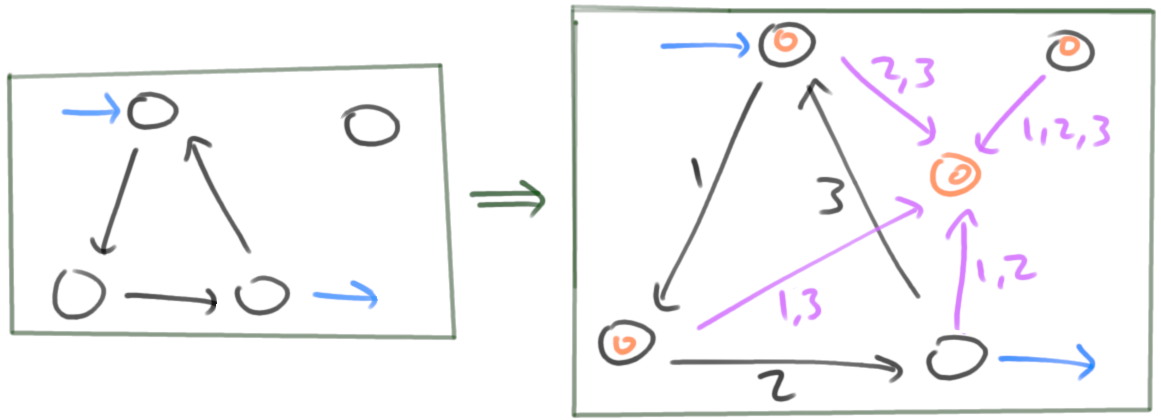
\includegraphics[width=10cm]{ALL_DFA_in_NL.png}
  \end{center}
  We will show that \(\textit{ALL}_{\textsf{DFA}}\)
  by proving \(\ol{\textit{PATH}} \logredu \textit{ALL}_{\textsf{DFA}}\).
  Suppose we have some instance \(\angles{G, s, t}\)
  of \(\textit{PATH}\) where \(G = (V, E)\).
  Consider the \textsf{DFA} \(M\) where the states are
  \(V \union q_A\) where \(q_A\) is a new accepting state.
  Moreover, everything except \(t\) is an accepting state.
  Label each each transition with its own symbol.
  Then, in order to make it a \textsf{DFA},
  all of the remaining edges will go to \(q_A\).

  If \(\angles{G, s, t} \in \ol{\textit{PATH}}\),
  then there is no way to get to the reject state,
  and \(M \in \textit{ALL}_{\mathsf{DFA}}\).
  Conversely, if \(\angles{G, s, t} \in \textit{PATH}\),
  there exists some sequence of edges (and therefore indices)
  that reach the non-accepting state,
  and \(M \notin \textit{ALL}_{\mathsf{DFA}}\).
\end{proof}




% the braces means that we'll do it if we have time, which means we won't do it


\end{document}

